\subsection{Kinect V2}
\label{subsec:kinectv2}

Kinect merupakan seri perangkat \emph{motion sensing input} yang dikembangkan oleh Microsoft dan pertama kali dirilis pada 2010.
Perangkat ini terdiri atas sebuah kamera RGB, pemancar dan detektor cahaya inframerah yang memetakan kedalaman menggunakan perhitungan \emph{time of flight}, sebuah mikrofon,
  beserta perangkat lunak dan kecerdasan buatan dari Microsoft yang memungkinkan perangkat ini untuk melakukan \emph{gesture recognition}, \emph{speech recognition}, dan \emph{body skeletal detection} pada satu hingga empat orang secara \emph{real-time}.

\begin{figure}[ht]
  \centering
  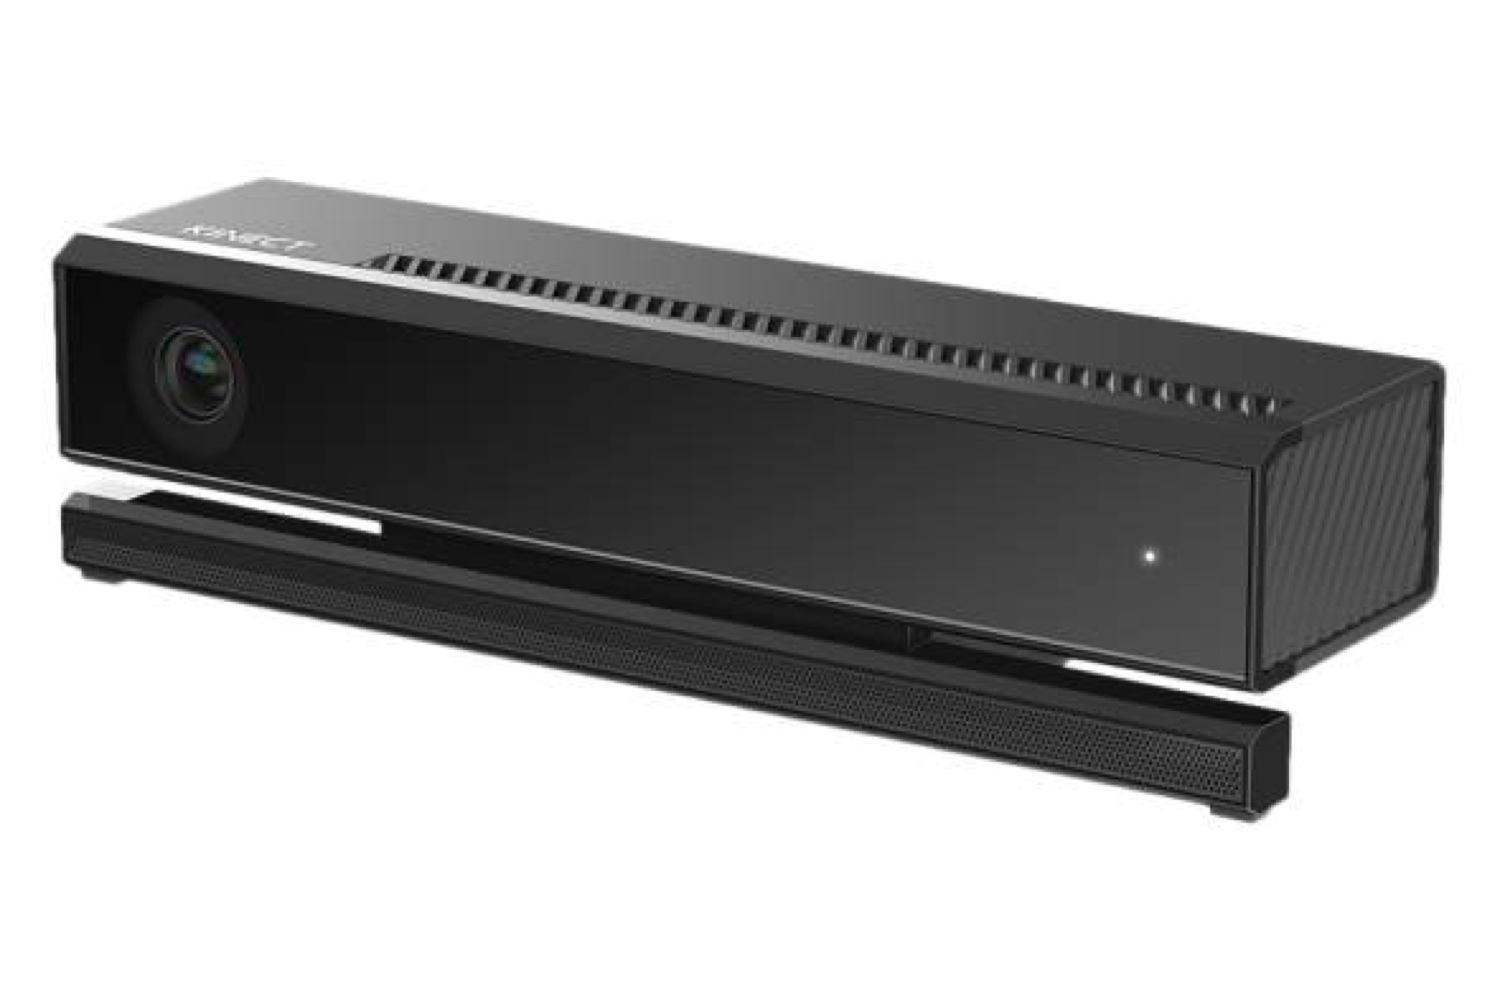
\includegraphics[scale=0.12]{gambar/kinect-v2.jpg}
  \caption{Perangkat \emph{depth camera} Kinect V2 \citep{url:kinectv2}.}
  \label{fig:kinectv2}
\end{figure}

Kinect V2 merupakan seri Kinect yang dirilis pada 15 Juli 2014 untuk sistem operasi Windows.
Perangkat ini dikembangkan dari Kinect untuk XBox One dan merupakan pengganti bagi Kinect untuk Windows yang awal.
Seperti yang terlihat pada gambar \ref{fig:kinectv2},
  Kinect V2 memiliki fitur yang sama dengan seri sebelumnya,
  yakni terdiri atas sebuah kamera RGB dan pemancar serta detektor cahaya inframerah yang memungkinkan perangkat ini untuk menghasilkan sebuah citra RGBD.
